\chapter{Graphs}
    \section{Definitions}
        \begin{definition}[Graph]
            A graph is a pair $G = (N, E)$, with $N$ a set of nodes (vertices) and $E \subseteq N x N$ a set of pairs of nodes.
        \end{definition}
        The intuitive representation is the classic web of interconnected nodes.\\
        There are two type of graphs, depending on how is possibile to traverse the edges:
        \begin{enumerate}
            \item \textbf{Undirected} graph $G = (N, E)$ with $E$ set of \textit{edges}, i.e. unordered pairs of nodes, denoted by $\{i, j\}$ for some $i, j \in N$.
            \item \textbf{Direct} graph $G = (N, A)$ with $A$ set of \textit{arcs}, i.e. ordered pairs of nodes, denoted by $(i, j)$ for some $i, j \in N$.
        \end{enumerate}
        Note the different name of the "edges/arcs" (and syntax) based on in which way is it possible to traverse them.
        \begin{definition}[adjacent nodes]
            Two nodes are said to be \textbf{adjacent} if there's an edge connecting them.
        \end{definition}
        \begin{definition}
            An edge $e$ is incident in a node $v$ if $v$ is an endpoint of $e$ .
        \end{definition}
        \begin{definition}
            \begin{itemize}
                \item[]
                \item[] \textbf{Undirected graphs}: The degree of a node is the number of incident edges
                \item[] \textbf{Directed graphs}: The \textit{in-degree (out-degree)} of a node is the number of arcs that have it as head (tail).
            \end{itemize}
        \end{definition}
        \begin{definition}[Path]
            \begin{itemize}
                \item[]
                \item[] \textbf{A path} from $v_1 \in N$ to $v_k \in N$ is a sequence of consecutive edges $p =  \{v_1 , v_2 \}, \{v_2 , v_3 \}, . . . , \{v_{k-1} , v_k \}$\\with $\{v_l , v_{l+1}\} \in E$ for $l = 1, . . . , k - 1$.
                \item[] \textbf{A directed path} from $v_1 \in N$ to $v_k \in N$ is a sequence of consecutive arcs $(v_l , v_{l+1}) \in E$, for $l = 1, . . . , k - 1$.
            \end{itemize}
        \end{definition}
        A \textbf{path} is a subset of the $E$ set composed of consecutive edges (the endpoint of an edge is the "start"point of the next one\footnote{not in a directional way! we are talking about non directed graphs, the two consecutive edges just in fact share an endpoint}) that connects some edges in the graph.
        \begin{definition}
            Two nodes are \textbf{connected} if exists a path that links them.
        \end{definition}
        \begin{definition}
            A graph con be \textbf{connected} to, if and only if there exists a path the connects \textbf{all its nodes}.
        \end{definition}
        \begin{definition}
            A graph is \textbf{directed} if some of the edges can be traversed in only one way. These edges are called \textbf{arcs}.
        \end{definition}
        \begin{definition}
            A \textbf{cycle} or \textbf{circuit} is a directed path that end where it starts.
        \end{definition}
        \begin{definition}
            \label{def:completeGraphDefinition}
            A graph is \textbf{complete} if for all pair of nodes there's an edge connecting them.
        \end{definition}
        Reasoning on the definition \ref{def:completeGraphDefinition}, we can calculate the upper bounds for the number of edges given the nodes: 
        \begin{equation}
            \begin{cases}
                e \leq \frac{n \times (n-1)}{2} \text{ if undirected} \\
                e \leq n \times (n-1) \text{ if directed}
            \end{cases}
        \end{equation}
        where intuitively "e" is the number of edges and "n" the number of nodes.\\
        Given this two inequalities, we can redefine completeness: 
        \begin{definition}
            a graph is complete if and only if $e = \frac{n \times (n - 1)}{2}$ or $e = n \times (n - 1)$ depending on the graph being directed.
        \end{definition}
        \begin{definition}
            Given an undirected graph $G = (N, E)$ we can take $S \subset G$ subsets of nodes; we then observe $\delta(S)$ the \textit{cut} induced by S is the subsets of \textbf{edges} that connects S to N \textbackslash S.
        \end{definition}
        \begin{figure}[H]
            \centering
            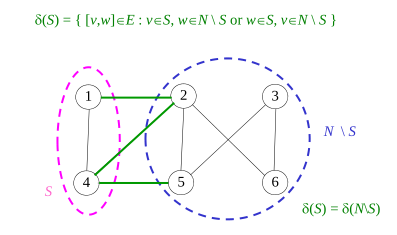
\includegraphics[width = \textwidth]{./images/Cut.png}
        \end{figure}
        Same definition holds for directed graphs, but this time we can distinguish among \textit{outgoing} and \textit{incoming} cuts, wheter the edges are all exiting S or ending in it.
        \begin{definition}
            A graph is said to be \textbf{bipartite} if we find a partition $N = (N_1, N_2)$ such as $\delta(N_i) = \emptyset$. So \textbf{the two subsets are disconnected}.
        \end{definition}
        A bit of foreshadowing: if a cut from a partial tree to another portion of the graph holds a minimum cost arc, then \textit{there exists a spanning tree with that arc}. This is called the \textbf{cut property}.
            
        \subsection*{Data Representations for Graphs}
            Depending one the edges / nodes ratio, two different data structures can hold a valid representation for a graph. When $e \approx n^2$ (a dense graph) then an adjacency matrix is the best choice. Otherwise (sparse graphs) linked lists of successors for each node.  

    \section{Graph reachability problem}
        The reachability problem can be formulated as "given a graph, determine all the nodes that are reachable from a starting one, decided a priori. A node is reachable is there's a path from the starting one and itself".
        
        To solve this problem, we can use the \textbf{breadth-first search algorithm}. 
        \begin{figure}[H]
        	\centering
        	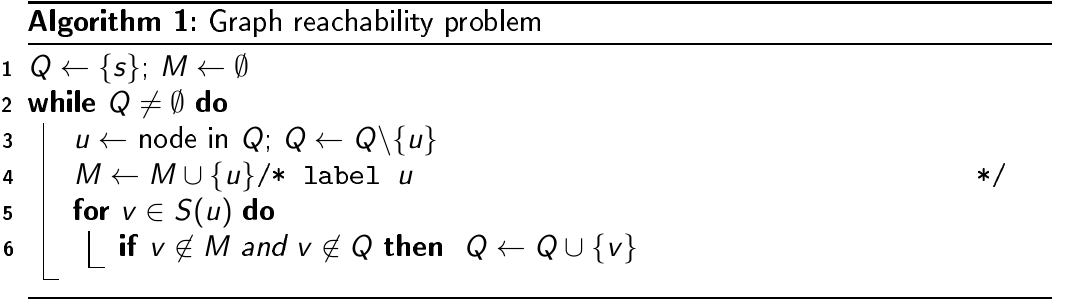
\includegraphics[width = \textwidth]{./images/breadth-first-search.png}
            \caption{Breadth-first search algorithm pseudo code}
            \label{fig:breadthFirstSearchPseudoCode}
        \end{figure}
        \textbf{Note}: Here $Q$ is managed as FIFO queue.
        \subsection{Complexity of the reachability algorithm}
            Refer to \ref{fig:breadthFirstSearchPseudoCode} image.
            
            At each iteration of the while loop:
            \begin{enumerate}
                \item Select one node $u$ in $Q$, extract it from $Q$ and insert it in $M$.
                \item For all nodes $v$ directly reachable from $u$ and not already in $M$ or $Q$, insert $v$ in $Q$.
                \item Repeat form 1.
            \end{enumerate}
            
            Since each node $u$ is inserted in $Q$ at most once and each arc $(u, v)$ is considered at most once, the overall complexity is
            $O(n + m)$, where $n = |N|$, $m = |A|$.\\
            \textbf{Note}: For dense graphs, $m = O(n^2)$.
    \section{Subgraphs, Trees, Spanning Trees}
        We call $G' = (N', E')$ a subgraph of $G = (N, E)$ if and only if
        \begin{equation}
            \begin{cases}
                N' \subseteq N \\
                E' \subseteq E \\
                \text{all edges inside $E'$ connects nodes in $N'$}
            \end{cases}
        \end{equation}
        \begin{definition}[Tree]
            A tree $G_t = (N', E')$ is a subgraph of a network that's both \textbf{connected} and \textbf{acyclic}.
        \end{definition}

        \textbf{Note}: A tree is \textit{spanning} if it contains all the nodes of the original graph. The \textit{leaves} of a tree are the nodes with unitary degree.

        Properties of trees:
        \begin{itemize}
            \item Every tree with a number of nodes greater than 2 has at least 2 leaves
            \item All trees have number of arcs equal to number of nodes minus 1
            \item Every pair of nodes in a tree is connected by a unique path (acyclic connected graph)
            \item By adding an edge to a tree, we create a \textit{unique cycle}. This also mean that if we now remove \textit{any} of the edges of this new unique cycle we go back to a spanning tree
            \item A complete Graph with n nodes has exactly $n^{n-2}$ spanning trees
        \end{itemize}

    \section{Minimum Cost Spanning Tree}
        \textbf{Problem}: find in a graph $G = (N, E)$ with \textit{weighted arcs}\footnote{numerated arcs with a "cost" associated to them} a subgraph that is a tree and has minimum total cost of edges.
        
        The \emph{minimum total cost} condition is verified when the sum of the costs along edges cannot be decreased by swapping edges in and out from the tree.
        
        \begin{theorem}[Cayley, 1889]
            A complete graph with $n$ nodes $(n \geq 1)$ has $n^{n-2}$ spanning trees.
        \end{theorem}
       

        \subsection{Prim's Algorithm}
            The Prim's algorithm is a simple iterative algorithm to build a spanning tree starting from an initial node.\\
            The algorithm adopts an incremental \emph{greedy}\footnote{A greedy algorithm constructs a feasible solution iteratively by
            making at each step a \emph{locally optimal} choice, without reconsidering previous choices.}
            strategy: it adds to the (initially empty) tree the nearest node every time (nearest = connected with the minimum cost outgoing edge) until the tree has the same number of nodes as the original graph.\\
            The algorithm
            \begin{itemize}
                \item Input: Connected $G = (N, E)$ with edge costs.
                \item Output: Subset $T \subseteq N$ of edges of $G$ such that $G_T$ = $(N, T)$ is a minimum cost spanning tree of $G$.
            \end{itemize}
            The Method:
            \begin{enumerate}
                \item initialize the output: $S = (N', T)$ where $N'$ is composed only of the initial chosen node and $T = \emptyset$ is the set of edges.
                \item add to S's nodes the "nearest" node from the ones connected to it, and add to T the lowest-cost edge. Careful: we are watching at \emph{}{all the nodes reachable from the outgoing cut of $S$}, not only the ones from a single node.
                \item repeat step 2 until the graph is covered.
            \end{enumerate}
            Prim's algorithm is \emph{exact}\footnote{Formally proven to provide an optimal solution for each instance of a problem}.\\
            This algorithm exploits the \textbf{cut property}.

    \section{Shortest Path and Shortest Path Trees}
        Finding the shortest path on a graph from node A to node B is another classical problem. The most used algorithm is the famous Dijkstra's algorithm.

        \paragraph{Dijkstra Algorithm}
            Dijkstra algorithm is similar to the Prim's one, but applied in a different direction. Dijkstra starts from a subset of the nodes (called the "unvisited nodes") and considers themone at a time. At each iteration, a node is selected from the unvisited set (the first is chosen a priori, will be the \textit{initial} node) and for all his neighbours is updated the distance. When all neighbours have been inspected, the node is marked as "visited"\footnote{and never checked again}. Next node to be selected is the \textit{closest} and the algorithm restarts. It finishes when the "unvisited" set is empty. More schematically:
            \begin{enumerate}
                \item Select the closest node (first one a priori)
                \item Check his neighbours and update their distance
                \item When all neighbours have been inspected, go to point one. If no more unvisited nodes exists, end.
            \end{enumerate}
            At the end of the algorithm we have a \textit{shortest path tree}\footnote{that's \underline{\textbf{different}} from a minimum cost spanning tree} that highlights all the shortest paths from the initial node to all other nodes in the graph. Taking the \textit{closest} node at each iteration checking the outgoing cut from the "visited nodes" set ensures the exactness of Dijkstra algorithm.

        \paragraph{Floyd Warshall Algorithm}
            Negative-cost edges, if present, do not allow to apply Dijkstra algorithm. But they are a further threat to shortest path problems: if a \textit{negative cost cycle} exists, there's no minimum cost path that's also finite between two nodes that traverse that cycle. This is a ill-defined problem, and the Floyd Warshall algorithm detects it. This algorithm uses two matrixes: a \underline{distance} and a \underline{predecessor} one. At each iteration of the algorithm, a \textit{triangular check} is performed: for all his neighbours, an undirect path is searched (a multi step path, generally with a single intermediate node) to shorten the distance wrt the direct path.
            \begin{enumerate}
                \item initialize a counter \emph{h} at 1, it will be our index for the nodes
                \item for each value of the counter from 1 to the number of nodes, perform the check $d_{ij}\, >\, d_{ih}\, +\, d_{hj}$ to evaluate if there is an alternative two-steps path that reduces the distance between nodes $i$ and $j$.
                \item if a loop with negative cost is detected (so a node can go from itself to itself with less than 0 distance passing through another node) that the problem is flagged as ill and the algorithm terminates
            \end{enumerate}
            At the end, combining the two matrixes, we have a shortest path tree of the original graph. This time, it can be calculated with negative cost arches.

        \subsubsection{Direct Acyclic Graphs and Dynamic Programming}
            If we add the hypothesis that the graph we're working on (to find the shortes path or the minimum cost spanning tree) does not contain cycles, we can study some more interesting solutions to such a problem. Moreover, DAGs\footnote{directed acyclic graphs} are well suited to model a wide range of problems.

            \paragraph{Topological Ordering}
                DAGs can be \textit{topologically ordered}, which means that we can label the nodes as if the graph represents an order relation between them (in the algebraic sense). The formal definition is that
                \begin{equation}
                    \forall (i, j) \in A\, |\, i\, <\, j
                \end{equation}
                where A is the set of edges. This looks like a trivial additional property to a graph, but having a \textit{strictly monotone ordering of nodes} is super helpful.\\
                To order nodes in such a way, however, the algorithm is quite simple:
                \begin{enumerate}
                    \item find a node with no incoming edges\footnote{the existence of such a node is proved by the acyclicity condition} and assign the smallest index available
                    \item remove the node from the graph and return to point 1
                \end{enumerate}
            
            \paragraph{Dynamic Programming}
                The "dynamic programming" approach has a bit of a confusing name. The underlying idea is that we can exploit a recursive relation between costs along a shortest path, using the "shortest subpath" property: given $\pi_{ij}$ shortest path $i \rightarrow j$ we can divide it in $\pi_{it} + c_{tj}$ where $\pi_{it}$ is the \textit{shortest subpath from i to t} and the second term is the cost of the last step. If we define $L(i)$ as the cost of the \underline{shortest path} from the initial node to node \emph{i} we have that
                \begin{equation}
                    L(t) = min\{ L(i)_{i \text{ predecessor of } t}\, +\, c_{it} \}
                \end{equation}
                This is a recursive relation that can be expanded to all nodes in the path. I'll put here the example by the professor:
                \begin{figure}[H]
                    \centering
                    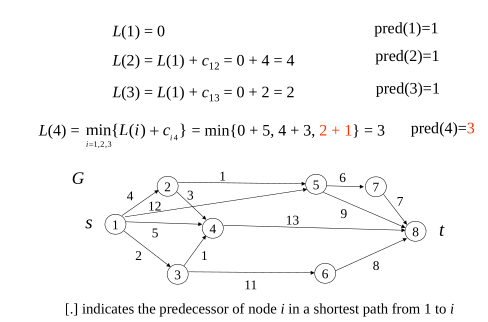
\includegraphics[width = \textwidth]{./images/DynProg.png}
                \end{figure}
                \begin{figure}[H]
                    \centering
                    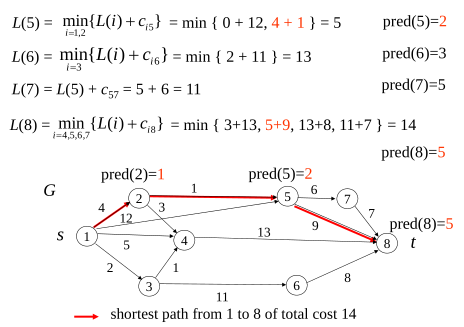
\includegraphics[width = \textwidth]{./images/DynProg2.png}
                \end{figure}


        \subsubsection{Project Planning}
            As shown in the Examples, we can use graphs to express dependency relationships. A direct application of this model is used when organizing various activitie inside a project: each phase will depend from some previous phases, there will be an "initial" phase with no predecessors and a final phase with no successors. The model adopted here is the one that represents
            \begin{itemize}
                \item \textit{activities} as arcs
                \item \textit{activity duration} with arcs weight
                \item \textit{checkpoints} as nodes
            \end{itemize}
            This formulation leads to a weighted directed acyclic graph. It's acyclic \textit{by nature}: it would be meaningless (and also logically incorrect) if activities in a project had circular relationships.\\
            This model helps in finding the \textit{minimum overall project duration}: being directed and acyclic, this will be the duration of the \textit{longest path} from the initial node to the final (we cannot compress the project time beyond that).

            \paragraph{Critical Path Method}
                The CPM aims to provide an optimal schedule for a project, with allotted time for each activity and the possible slack of each one, given the DAG of a project activities precedences. The algorithm is:
                \begin{enumerate}
                    \item Construct the DAG of activities and precedences
                    \item Topologically sorts the nodes
                    \item For each node, calculate
                        \begin{itemize}
                            \item The earliest start time starting from inital activity. This would be (at the final node) the minimum overall project duration
                            \item The latest time an activity can be started to NOT increase the minimum project duration (starting from the end, this time)
                        \end{itemize}
                    \item For each activity now we can calculate the \textit{slack}: $T_{max} - T_{min} - d$ where \emph{d} is the duration of the activity itself
                \end{enumerate}
                The slack of each activity indicates if it could be \textit{deliberately delayed} without affecting the overall project duration. There exist activities with null slack: these are called \underline{critical activities} and cannot be delayed in any case. They compose the critical path from the beginning to the end of the project.
        
        \subsubsection{Network Flows}
            Network flows problems are the ones that involves "distribution of a given resource over a network". Needless to say, they boils down to find the optimal throughput of a network given its \textit{Directed Weighted Graph} representation. In this kind of problems, we can remove the acyclicity hypothesis. The graph model we're dealing with is like:
            \begin{figure}[H]
                \centering
                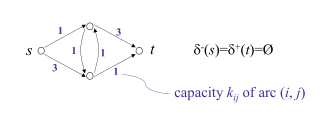
\includegraphics[width = \textwidth]{./images/Flows.png}
                \caption{Arcs weights assume a different meaning here: they are not more a cost or a lenght, but instead a \textit{width} or \textit{capacity} as shown in the blue note}
            \end{figure}
            We introduce the \textit{feasible flow vector}: it's a tuple of values representing the \textbf{occupated fraction} of each edge of the network; it should respects two major constraints:
            \begin{enumerate}
                \item Capacity constraints: $\forall (i, j) \in E\, |\, (0\, \leq\, x_{ij}\, \leq\, k_{ij} )$ where $x_{ij}$ is the value of the flow in the feasible flow vector, $k_{ij}$ the maximum capacity for that arc and \emph{E} the set of edges;
                \item Flow balance constraints: $\forall h \in N\, |\, (\sum(x_{ih}) = \sum(x_{hj}))$ that simply states that for each node, the amount that enters the node is the same amount that exits it
            \end{enumerate}
            We can then calculate the \textit{value of flow} $\phi = \sum(x_{sj})$, where \emph{s} is the initial node and j all the nodes reached by the \textit{outgoing cut} of \emph{s}; this represents the actual maximum flow that can go through the network.\footnote{The maximum flow is directly associated with the minimum capacity of a cut. Will see later how these, in fact, are mathematically correlated: \textit{they're dual problems}, or two representations of the same problem.}

            \paragraph{Ford Fulkerson's Algorithm}
                Another algorithm, this time to resolve a network flow problem. Again, this is just the algorithmic version of the intuitive solution for this problem: keep sending stuff on non-saturated channels until the network is maxed out.\\
                Said so, we need some additional definition to handle easily this algorithm:
                \begin{itemize}
                    \item a \textit{backward arc} is an edge of the network that "sends units backward" with regard to a simil-topological ordering of the nodes. We can "flat out" the graph of the network to visually understand what a backward arc is:
                        \begin{figure}[H]
                            \centering
                            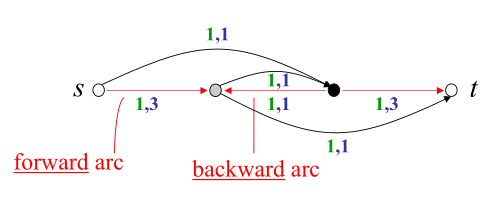
\includegraphics[width = \textwidth]{./images/BackwardArcs.png}
                        \end{figure}
                    \item an \textit{augmenting path} (wrt the current $\phi$) is a path through all the network (so start to end) where
                        \begin{equation} 
                            \begin{cases}
                                x_{ij}\, <\, k_{ij} \text{ for all forward arcs}\\
                                x_{ij}\, >\, 0 \text{ for all backward arcs}
                            \end{cases}
                        \end{equation}
                    \item the \textit{residual network} of a graph is a graph itself buil keeping track of the possible changes that can be applied to the flows on the arcs. This means, if we have a \underline{saturated channel} with capacity 3 we will have in the residual network the same channel but \textit{reversed}: this signals that we have a residual capacity of 3 units \textit{in the opposite direction}.
                        \begin{figure}[H]
                            \centering
                            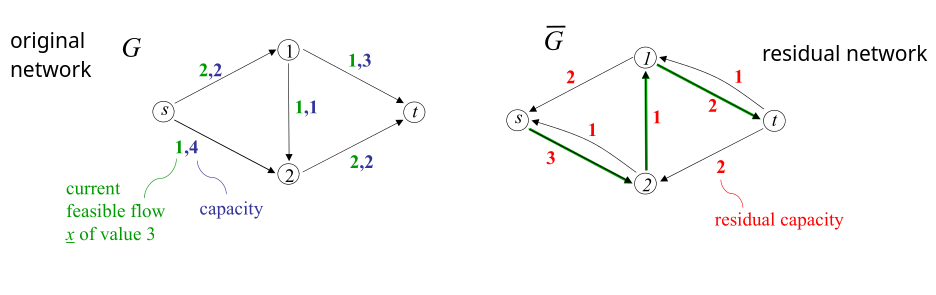
\includegraphics[width = \textwidth]{./images/Residual.png}
                        \end{figure}
                \end{itemize}
                So, the algorithm is structured in 2 main phases:
                \begin{enumerate}
                    \item Search for an augmenting path on the actual graph, then rebuild the residual graph. Repeat this point until no more trivial augmenting path can be found
                    \item Look for an augmenting path \textit{on the residual graph}. Using the second graph is useful when some edges could be desaturated in order to maximize the flow. The algorithm stops when on the residual graph there are no more paths from \emph{s} to \emph{t}
                \end{enumerate}